\chapter{Modélisation et analyse de la réalisation d'une opération}
Nous allons dans un premier temps réaliser une modélisation par réseau de Petri temporel de la réalisation d'une opération. Cette modélisation sera générique à la réalisation de toute opération $O_i$. Ensuite, nous réaliserons un code C qui permet d'estimer les durées des différentes opérations. Finalement, nous analyserons le réseau de Petri à l'aide de \emph{TINA 2.8.4}.

\section{Modèle réseau de Petri temporel d'une opération}
Nous avons, pour modélisation générique d'une opération, considéré que le chariot de déplacement se trouve en bas. Voici le réseau de Petri temporel (voir figure \ref{fig:RdPTempo_generique}) : \\
\begin{figure}[!ht]
\centering
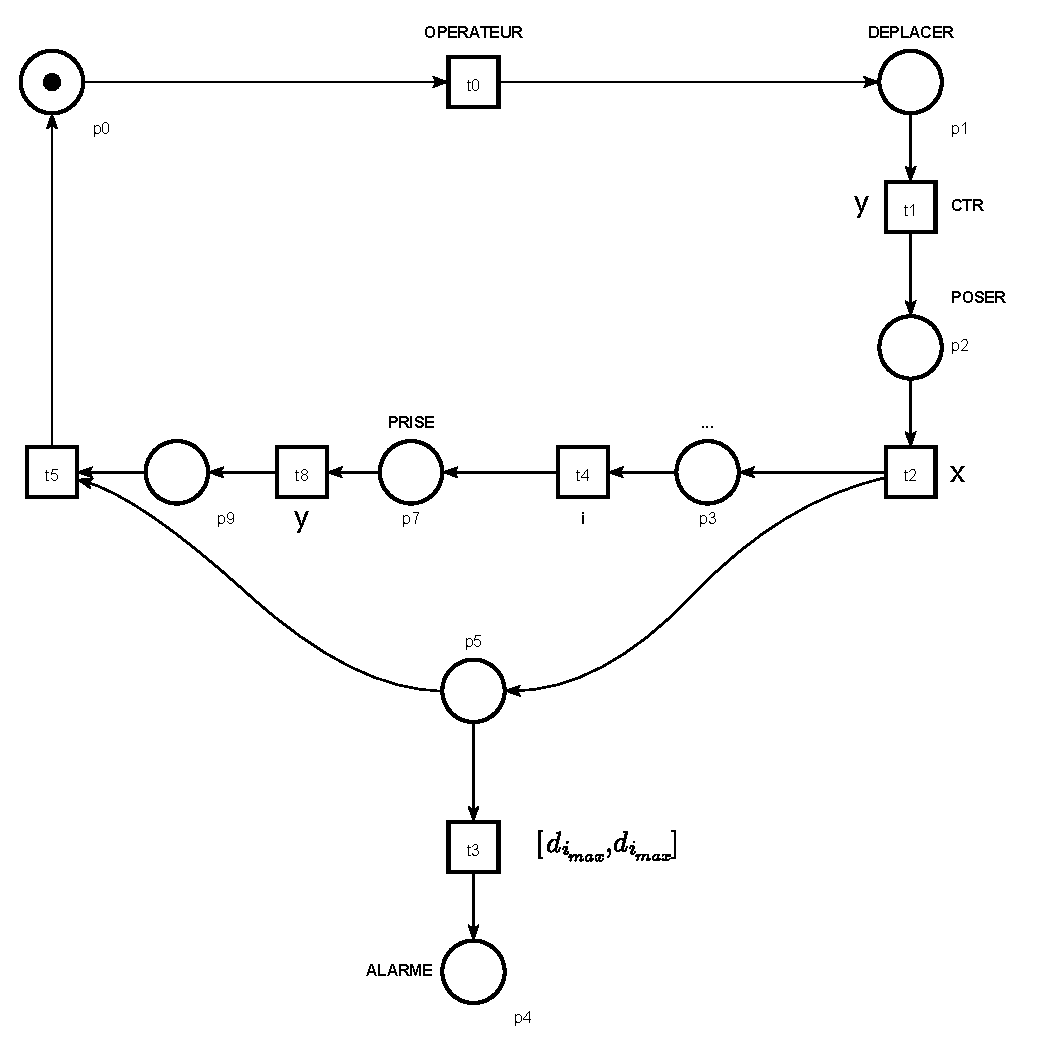
\includegraphics[width=.57\textwidth]{./I/images/III-1_v3.pdf}
\caption{\label{fig:RdPTempo_generique}Modèle réseau de Petri générique d'une opération.}
\end{figure}


Nous considérerons que l'action \emph{DEPLACER()} et l'événement \emph{FinDeplacer} correspondent à, respectivement, \emph{AVANCER()} et \emph{FinAvancer} si le chariot est à droite de l'emplacement de l'opération $o_i$  ou \emph{RECULER()} et \emph{FinReculer} si celui-ci est à gauche.


Le marquage initial est constitué d'un unique jeton sur la place $p_0$. Ce jeton, une fois que la transition $t_0$ est sensibilisée et tirée (pour cela il faut que l'événement \emph{OPERATEUR()} est eu lieu), est en $p_1$. Le chariot se déplace tant qu'il y a un jeton en $p_1$. Le jeton reste en $p_1$ jusqu'à ce que le charriot arrive à destination, c'est-à-dire que \emph{FinDeplacer} se déclenche. Lorsque cet événement ce produit, la transition $t_1$ est sensibilisée et tirée (le déplacement prend un temps $y$ qui est représenté sur la transition $t_1$). Ensuite, un jeton marque la place $p_2$ ce qui déclenche l'action \emph{POSER()}. Cette action prend un temps $x$ et celui-ci est représenté sur la transition $t_2$. Une fois le temps $x$ écoulé, la transition $t_2$ est tiré et les places $p_3$ et $p_6$ sont marqués d'un jeton chacun. 

À partir de cet état, il y a deux jetons dans le réseau : un permet de décrire le comportement du chariot et un autre, celui qui marque $p_6$, permet de déclencher l'alarme si la pièce qui subit l'opération $o_i$ n'est pas reprise avant le temps maximal de l'opération.  En effet, le jeton présent en $p_6$, au bout d'un temps $d_{i_{max}}$, va être consommé par la transition $t_6$ et un jeton va marquer $p_7$. Ceci déclenchera l'action \emph{ALARME()}.
Il faut donc que le jeton présent en $p_3$ arrive en $p_5$ en moins de $d_{i_{max}}$ unités de temps pour que l'alarme ne se déclenche pas. De cette façon, le tir de la transition $t_5$, qui nécessite et consomme un jeton en $p_6$ et un jeton en $p_5$, empêchera l'alarme de sonner et permettra d'effectuer une nouvelle opération (retour au marquage initial). 
La place $p_3$ à un événement \emph{...}, cela représente la possibilité d'effectuer n'importe(s) quelle(s) action(s) et de revenir à l'emplacement de l'opération $o_i$, de façon à ce que l'action en $p_4$, \emph{PRISE()}, de durée $y$, permette de récupérer la pièce. La transition $t_3$ est marquée de la temporisation $i$. Celle-ci représente le temps de(s) action(s) de la place $p_4$ et/ou un temps d'attente afin que l'on récupère la pièce à la fin de l'opération $ç_i$. Ainsi, si l'on souhaite que l'alarme ne sonne pas, il faut que $i + y < d_{i_{max}}$.

\section{Estimation de Prise/Pose et Avance/Recule}
\begin{center}
\textit{Voir annexe \ref{Annex:MesuresXY}, page \pageref{Annex:MesuresXY}.}
\end{center}
Nous avons maintenant besoin d'identifier le temps de \emph{AVANCER()} (égal à celui de \emph{RECULER()}) que l'on appelait précédemment$y$  et de \emph{PRISE()} (équivalent à celui de \emph{POSE()}) appelait $y$. Pour cela, nous avons créer, à partir d'un code fourni, un code permettant de mesurer les temps $x$ et $y$. Pour mesurer le temps d'une action, nous avons stocké le temps du PC à l'instant du début de l'action, puis nous avons stocké le temps à la fin de celle-ci et avons affiché la soustraction des deux temps sur le terminal. 
Nous avons déterminé que :
\begin{eqnarray}
x &=& \begin{bmatrix}
1 & 1
\end{bmatrix} \text{seconde}\\
y &=& \begin{bmatrix}
3 & 3
\end{bmatrix} \text{secondes}\\
\end{eqnarray}
\section{Analyse du modèle}
Grâce aux mesures précédentes, nous avons pus remplacer $x$ et $y$ par des valeurs temporelles sur le modèle générique. Nous avons choisi arbitrairement les valeurs de $d_{i_{min}} = 13$ secondes et $d_{i_{max}} = 16$ secondes, respectivement le temps minimal de l'opération et le temps maximal de l'opération $o_i$.  Ainsi, nous avons la condition suivante qui doit être respectée $i <d_{i_{max}}-y$, soit $i < 13$ secondes. Donc il "reste" moins de 13 secondes afin de réaliser d'autres opérations. Nous allons fixer une temporisation  $i=\begin{bmatrix}
12& 12
\end{bmatrix}$ secondes pour étudier le réseau. 

Figure \ref{fig:RdPTempo_generique_indentif}, voici le nouveau réseau de Petri temporel.
\begin{figure}[!ht]
\begin{minipage}[t]{.4\textwidth}
\centering
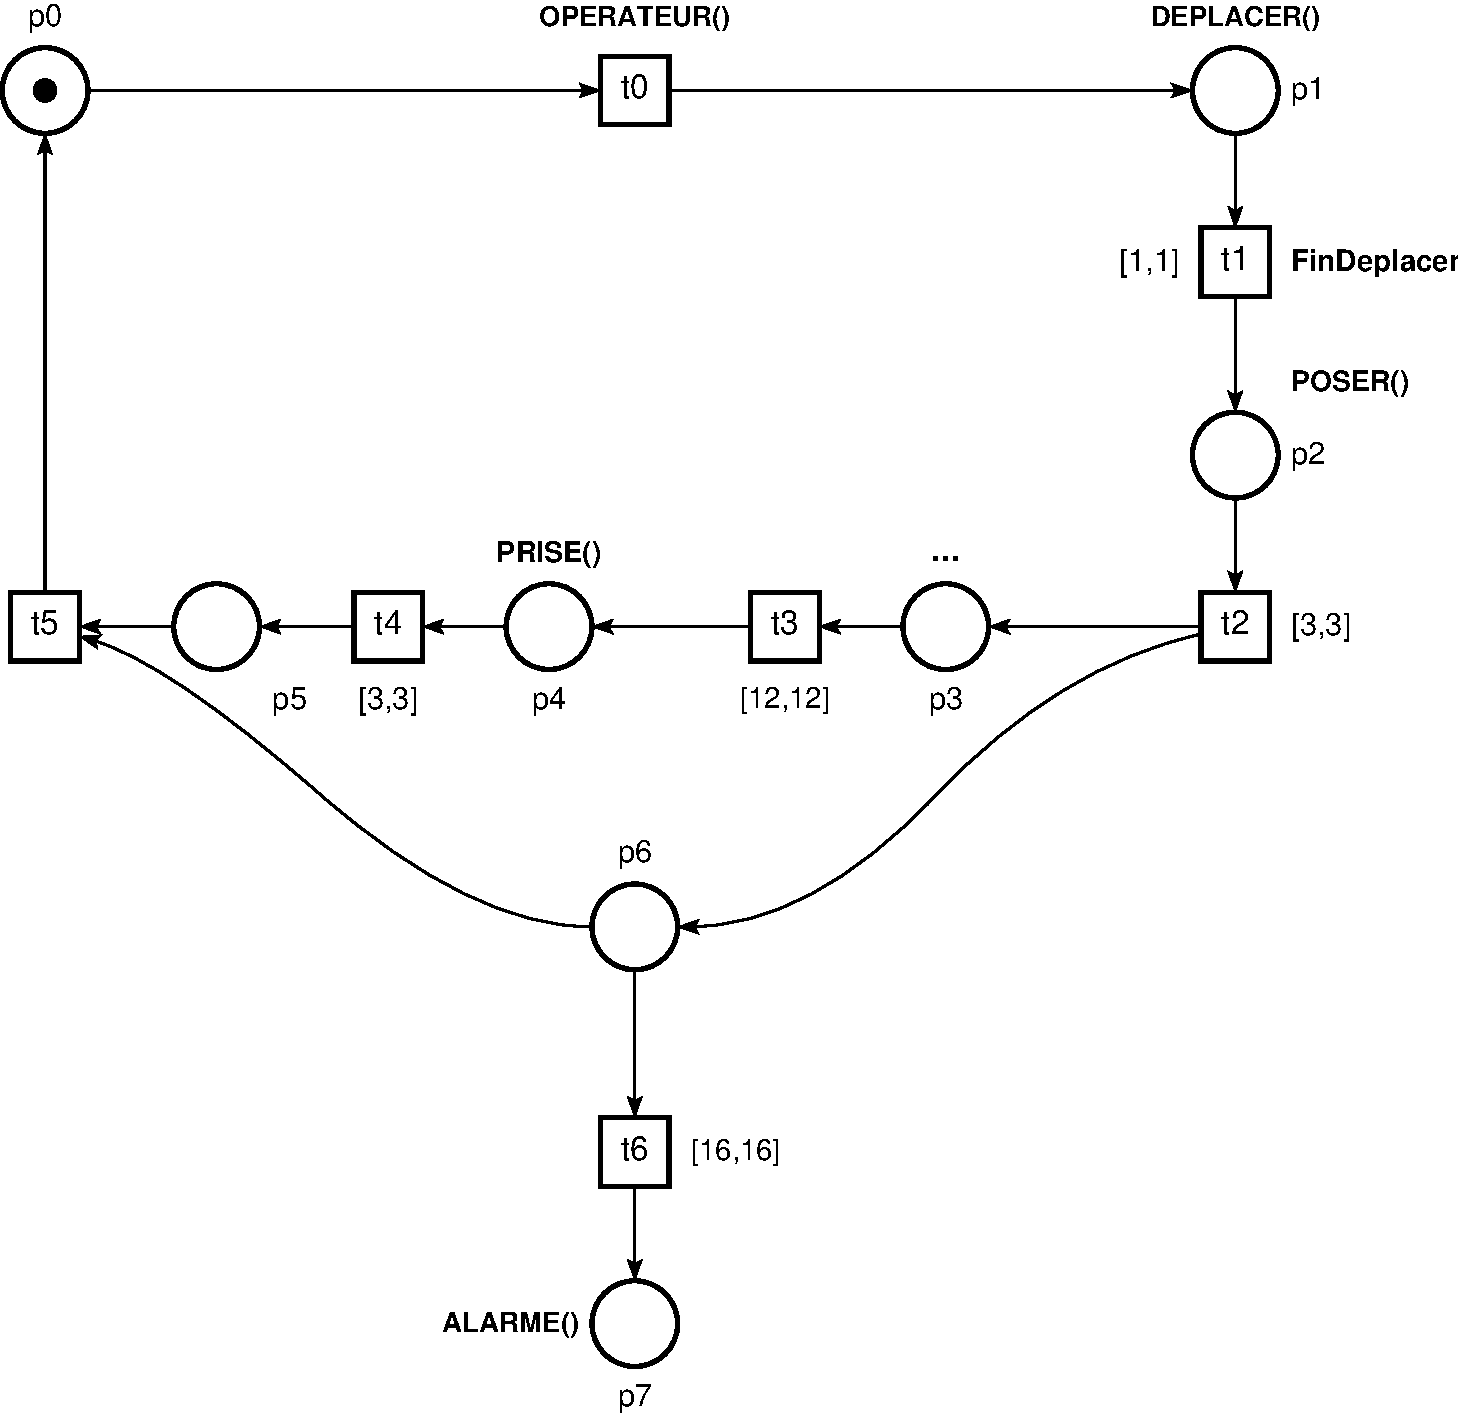
\includegraphics[width=.8\textwidth]{./I/images/III-1_v3_esti.pdf}
\caption{\label{fig:RdPTempo_generique_indentif}Modèle réseau de Petri générique d'une opération avec les temps estimés}
\end{minipage}\hfill%
\begin{minipage}[t]{.58\textwidth}
\centering
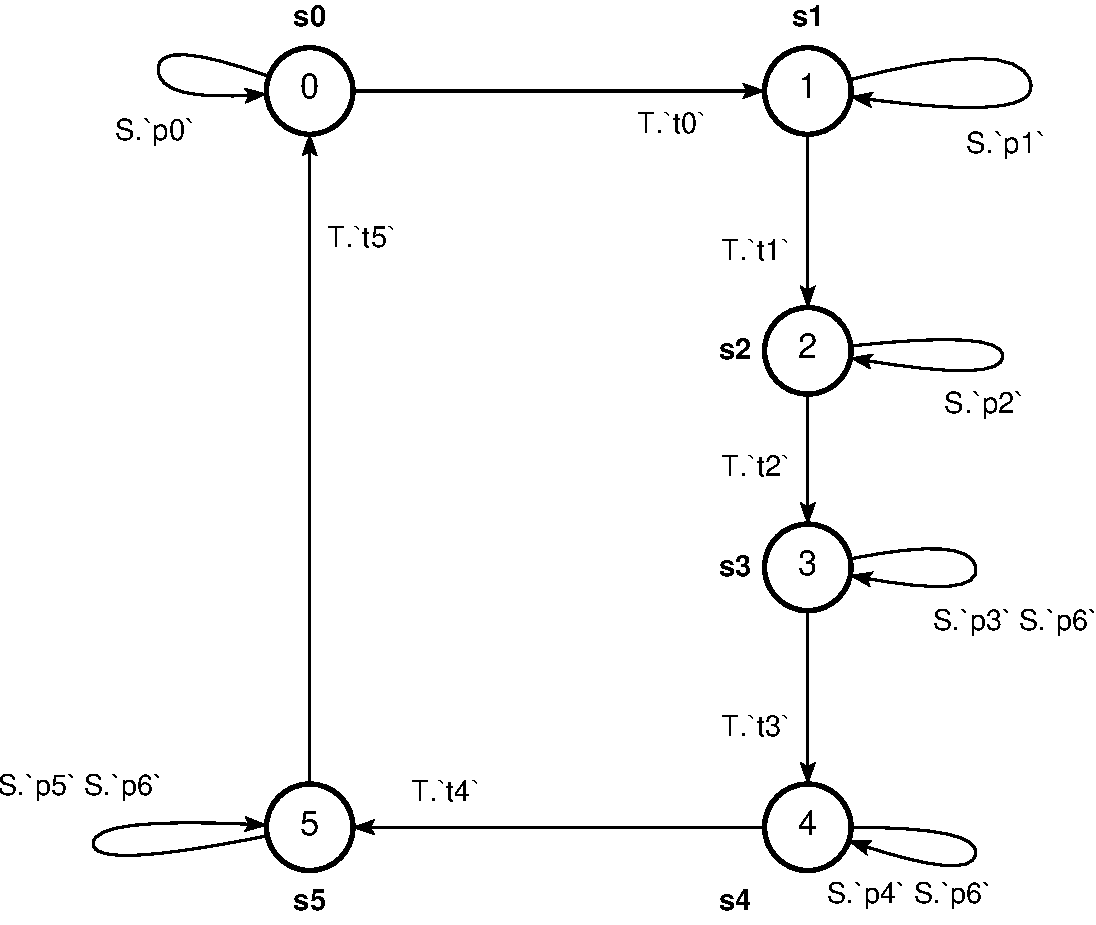
\includegraphics[width=.9\textwidth]{./I/images/III-1_v3_aut.pdf}
\caption{\label{fig:III-1-automate}Diagramme de classe.}
\end{minipage}
\end{figure}
Une analyse à l'aide de TINA nous a permis de déterminer les différentes classes du réseau. L'automate est présenté figure \ref{fig:III-1-automate}. Nous avons put aussi extraire les propriétés suivantes grâce à TINA.

\begin{itemize}
\item Le RdPT (Réseau de Petri Temporisé) n'est pas vivant. 
\item La transition $t_6$ est non vivante. 
\item LE RdPT est borné.
\end{itemize}

